\clearpage

\section{Simulation Analysis}
\label{sec:simulation}

Results that were asked for:

\begin{figure}[h] \centering
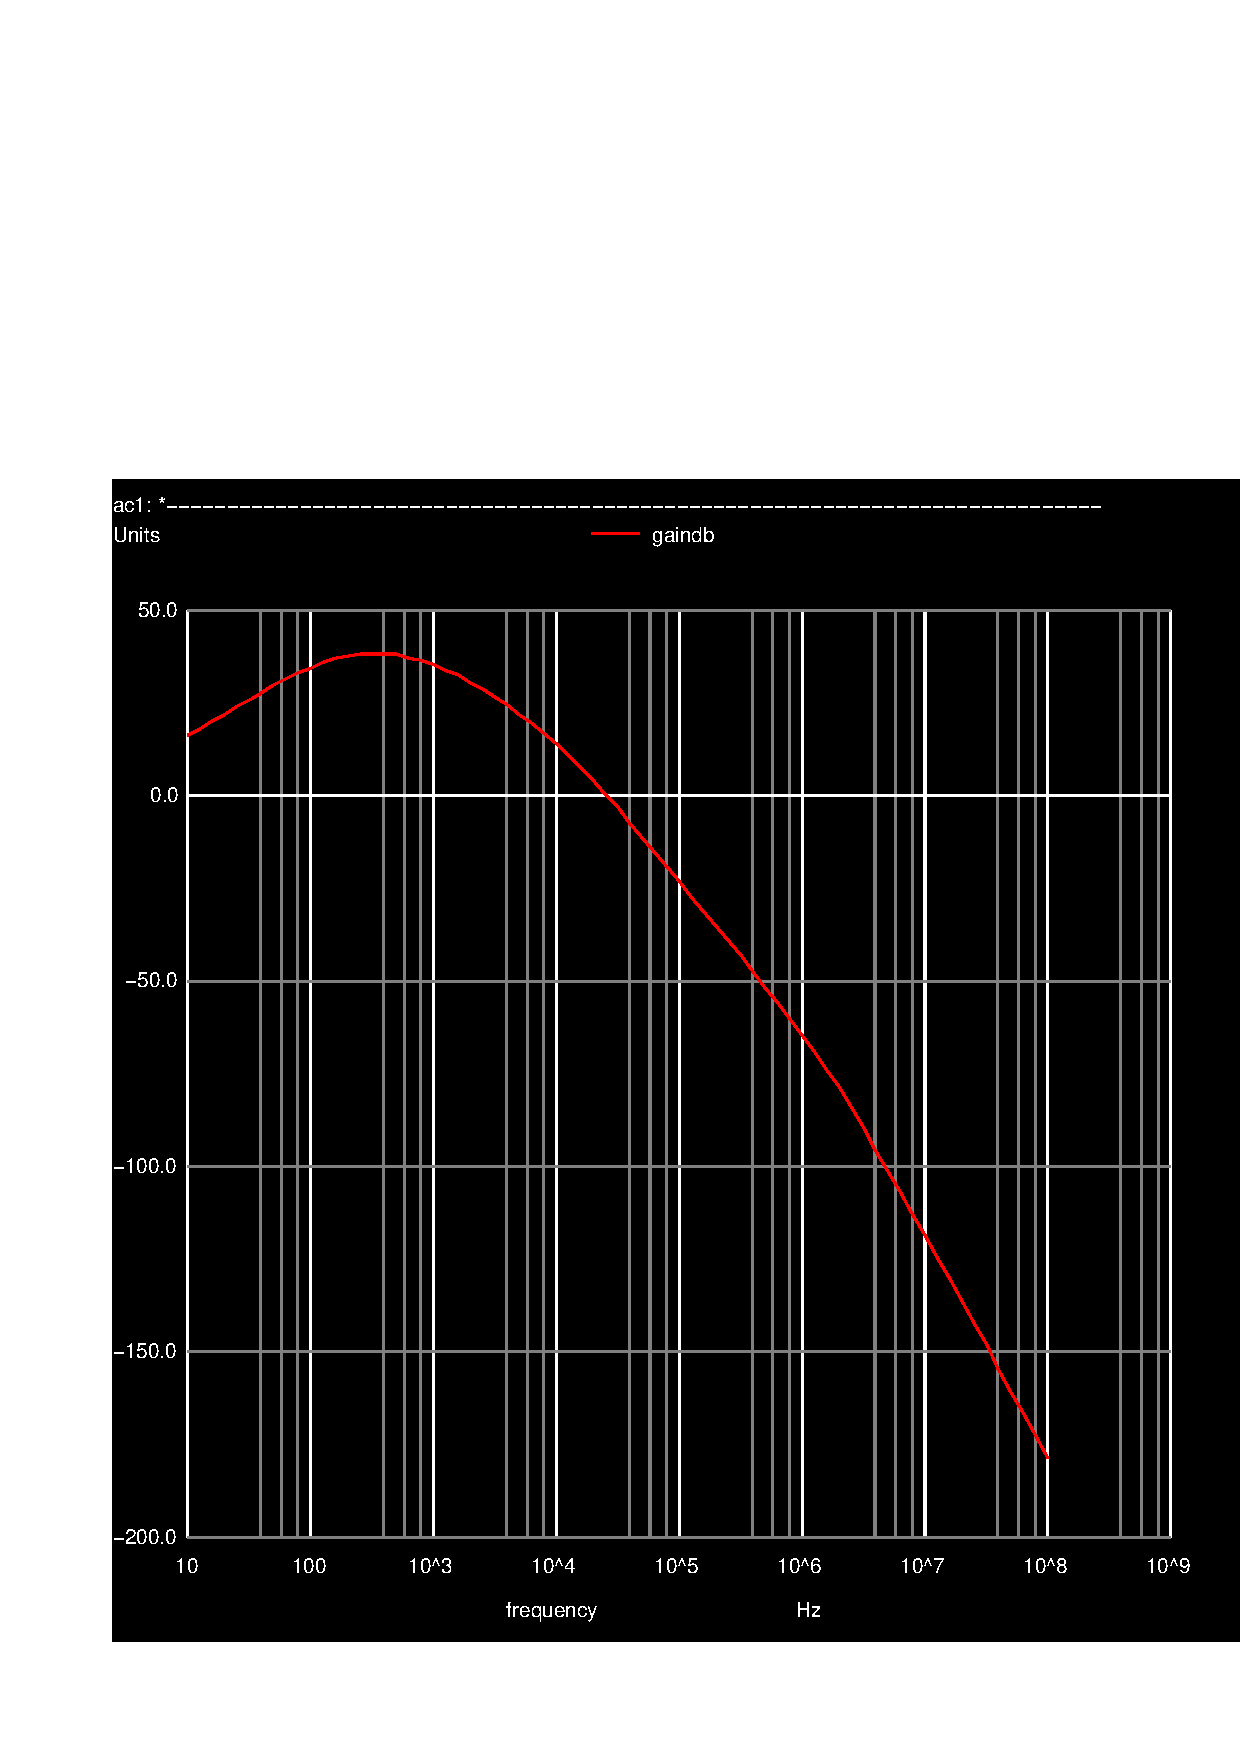
\includegraphics[width=0.5\linewidth]{../sim/gain.pdf}
\caption{Output Voltage Gain Simulated}
\label{fig:sim-gain}
\end{figure}

\begin{figure}[h] \centering
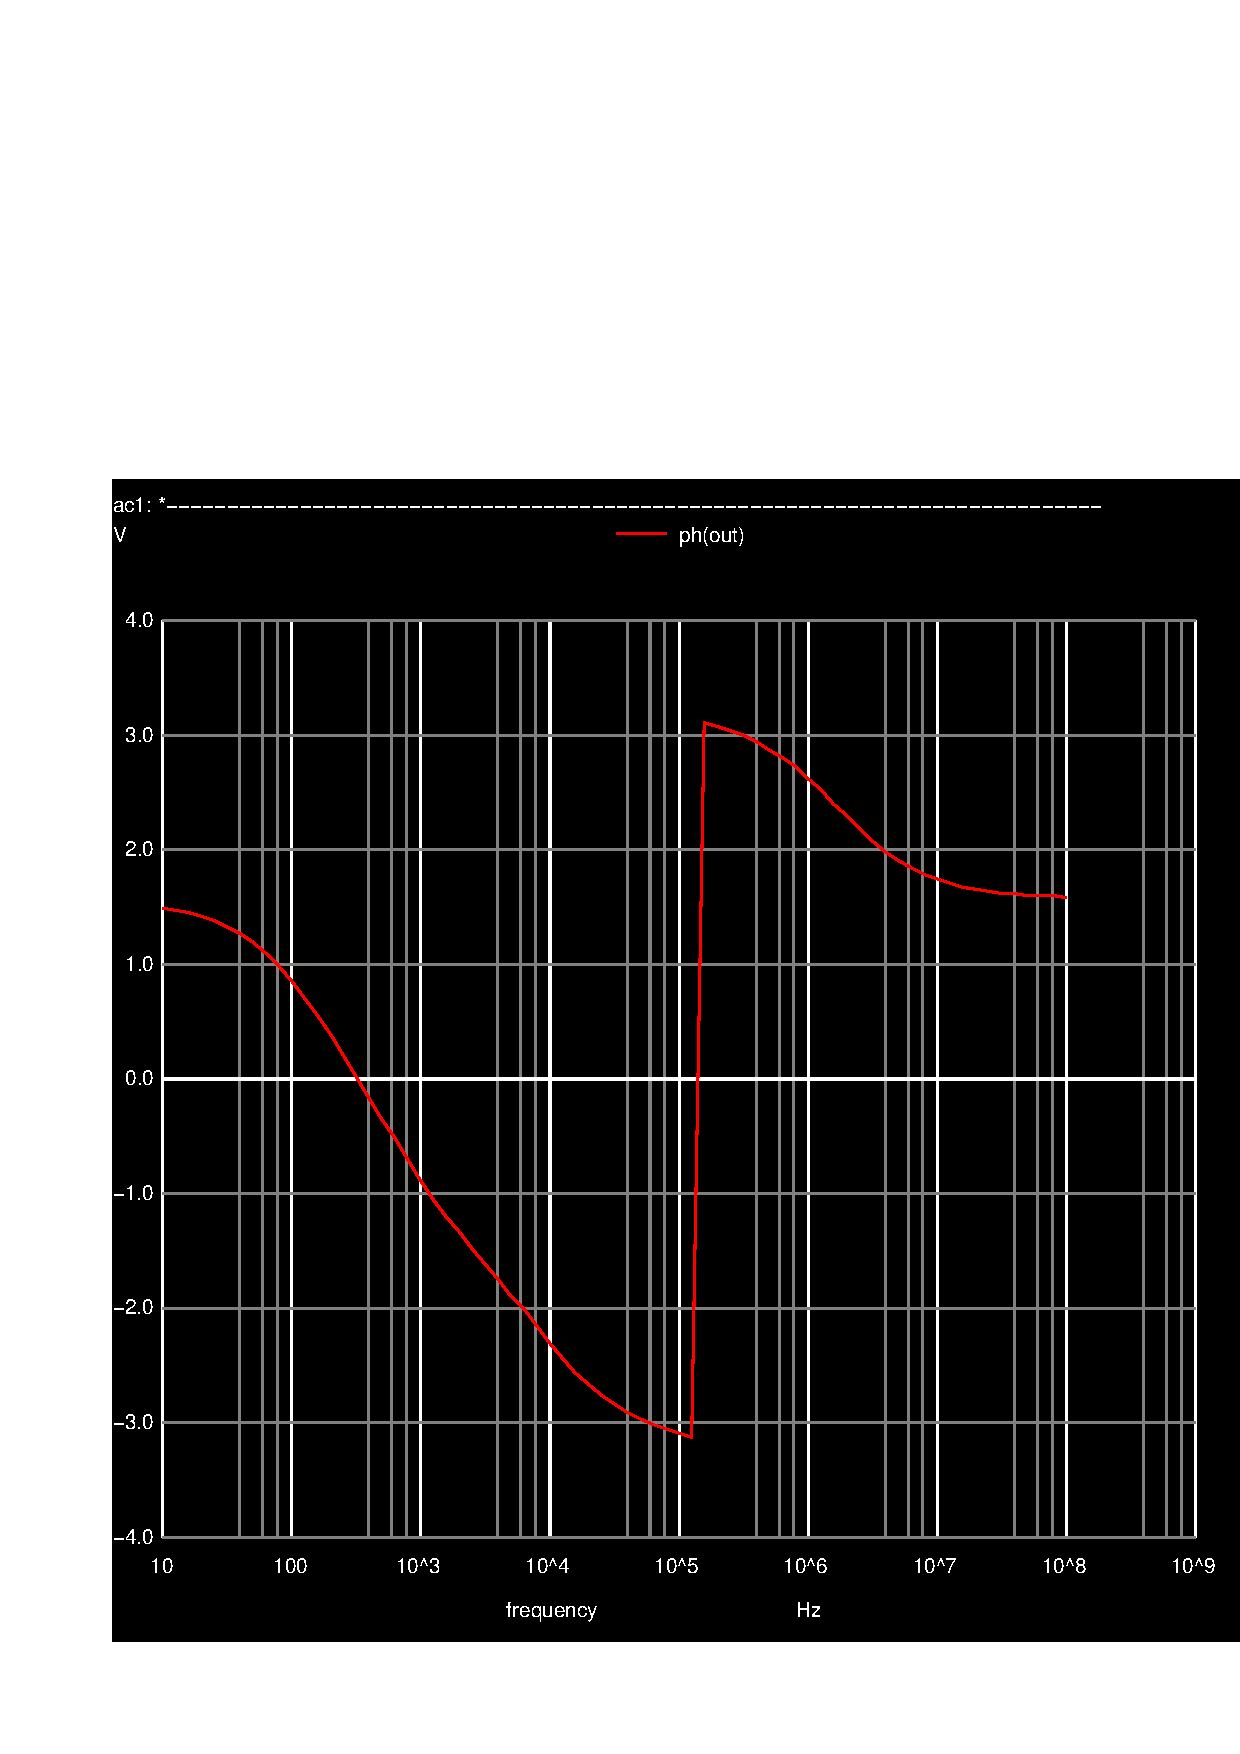
\includegraphics[width=0.5\linewidth]{../sim/phase.pdf}
%\caption{Output Voltage Gain Simulated}
%\label{fig:sim-gain}
\end{figure}

\begin{center}
\begin{tabular}{|l|r|}
  \hline    
  {\bf Variable} & {\bf Value ($\Omega$)} \\ \hline
  zin & 9.999982e+02,-3.99820e+02\\ \hline

\end{tabular}
\end{center}

\subsection{Output Impedance Calculation}

For us to be able to calculate the output impedance, we had to create a new circuit, similar to the original one. However, in this new circuit, that is displayed in Figure \ref{fig:circuit-out}, we have turned off the input voltage source and substituted the load for that same source.

\begin{figure}[h] \centering
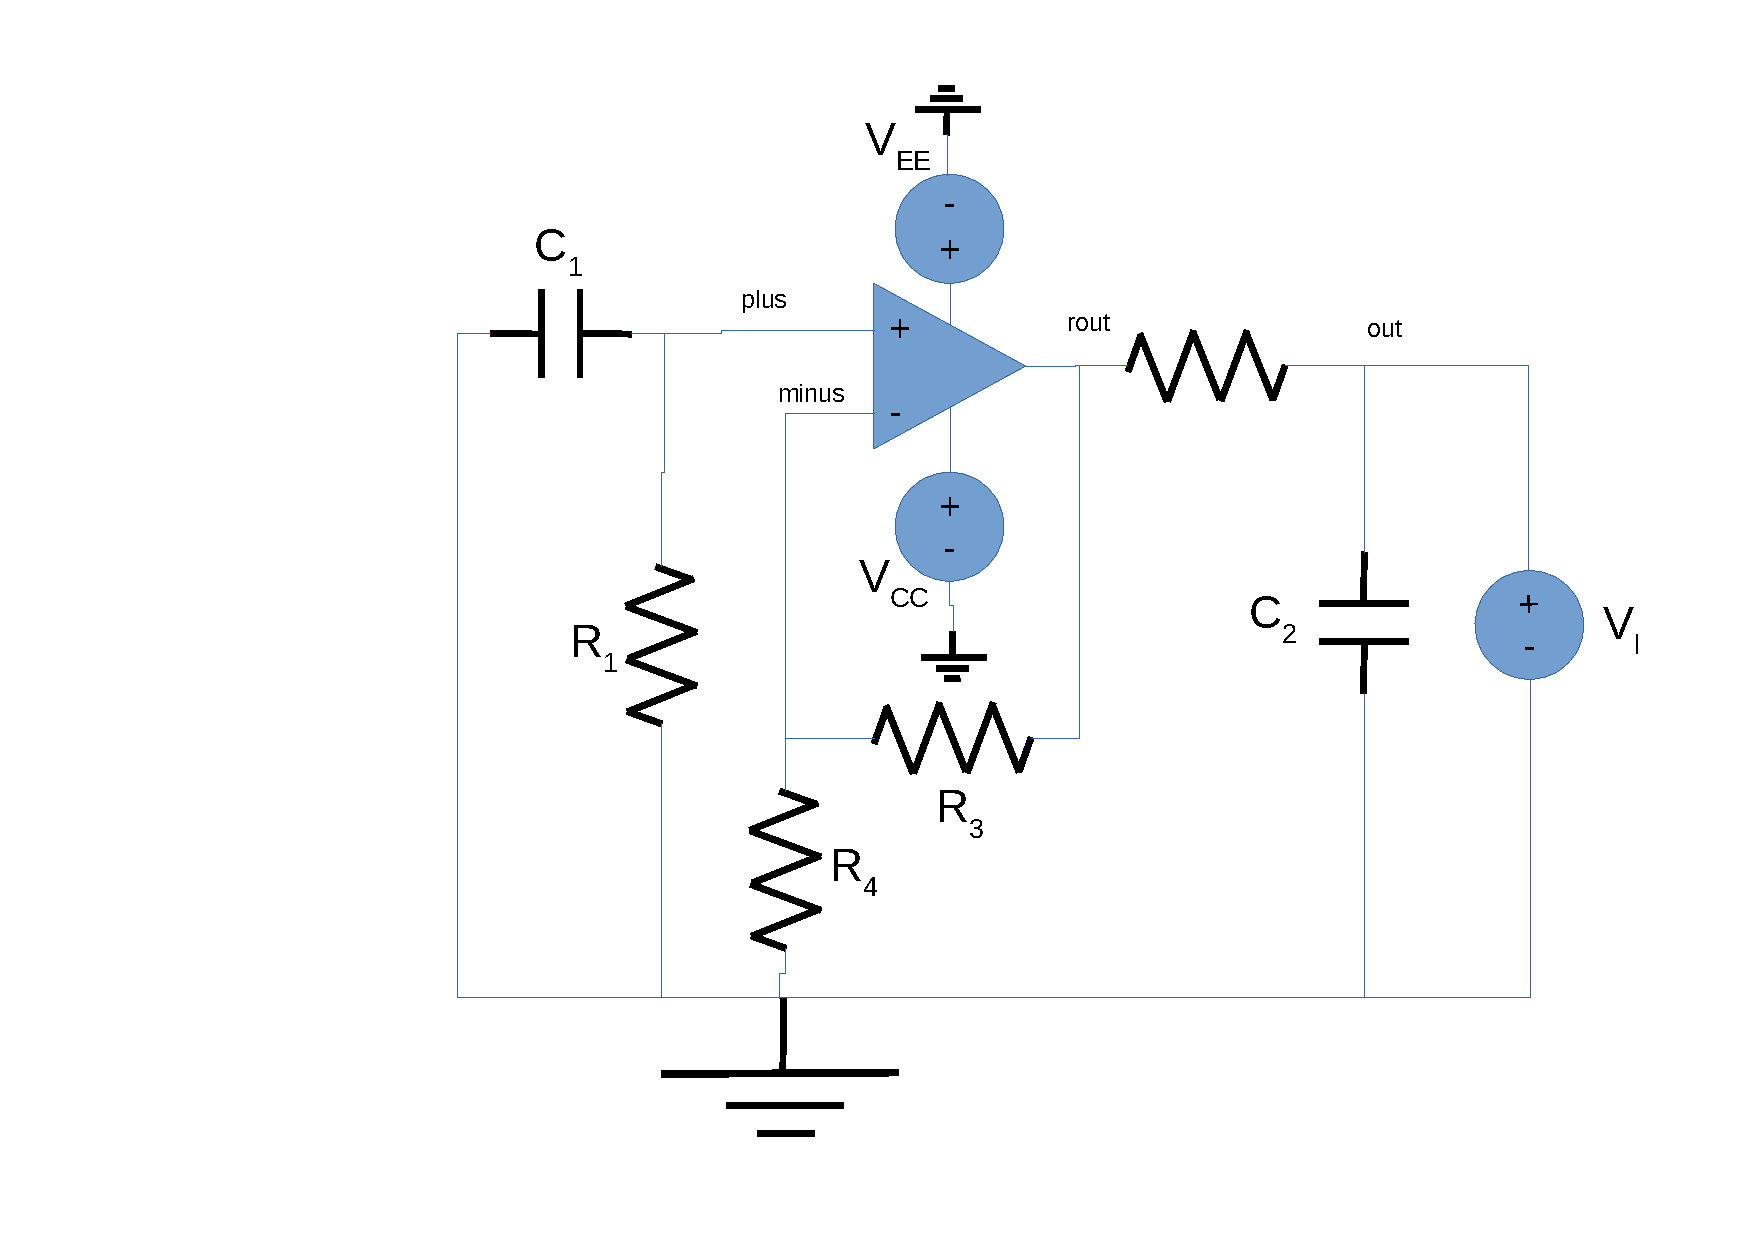
\includegraphics[width=0.6\linewidth]{circuit-out.pdf}
\caption{The circuit used to calculate the output impedance.}
\label{fig:circuit-out}
\end{figure}

\begin{center}
\begin{tabular}{|l|r|}
  \hline    
  {\bf Variable} & {\bf Value ($\Omega$)} \\ \hline
  zout & 8.011868e+02,-3.99270e+02\\ \hline

\end{tabular}
\end{center}

\begin{center}
\begin{tabular}{|l|r|}
  \hline    
  {\bf Variable} & {\bf Value (MU)} \\ \hline
  opampcost & 1.332329e+04\\ \hline
cost & 1.342749e+04\\ \hline

\end{tabular}
\end{center}

Relevant results:

\begin{center}
\begin{tabular}{|l|r|}
  \hline    
  {\bf Variable} & {\bf Value (dB)} \\ \hline
  gaindbmax & 3.834218e+01\\ \hline

\end{tabular}
\end{center}

\begin{center}
\begin{tabular}{|l|r|}
  \hline    
  {\bf Variable} & {\bf Value (Hz)} \\ \hline
  f1 & 1.165730e+02\\ \hline
f2 & 9.936323e+02\\ \hline
bandwidth & 8.770593e+02\\ \hline
cenfreq & 3.403391e+02\\ \hline

\end{tabular}
\end{center}

\begin{center}
\begin{tabular}{|l|r|}
  \hline    
  {\bf Variable} & {\bf Value} \\ \hline
  merit & 5.223670e-02\\ \hline

\end{tabular}
\end{center}